
\subsection{Science Objectives}
\label{sec:science}

\vspace{-0.05in}

\comred{5 pages for all science goals including the (temporary) two sections below.}

\subsubsection{The Inflationary Gravity Wave Background}

\vspace{-0.05in}

\comred{The verbiage below is taken from another proposal. Here we need to explain what are the science objectives 
of the CMBProbe, how the science objectives relate to the current state of knowledge, and to NASA's goals}
% Lloyd, Sarah, Dan, Rafael

The paradigm of inflation~\cite{guth81,linde82,albrecht82,sato81,kolb94}
%, in which the Universe underwent exponential expansion within the first $\sim$$10^{-35}$~sec, 
makes several predictions that are consistent with all current astrophysical 
measurements~\cite{spergel06,Tegmark:2006az,planck2015parameters,planck2015inflation}. 
A robust prediction of inflation is the existence of a stochastic background of gravitational radiation 
with an amplitude depending on the mechanism driving the accelerated 
expansion~\cite{starobinsky82,starobinsky83a,rubakov82,grishchuk75,abbott84a}.
In most scenarios, this `inflationary gravity wave background' (\igb) is predicted
to have a spatial power spectrum whose amplitude is proportional to the energy
scale of inflation $V^{1/4}$ via
$V^{1/4} = 3.7 \times 10^{16} \ r^{1/4}\,\, {\rm GeV},$
where $V$ is the inflaton potential and $r$ is the ratio of the temperature
quadrupoles produced by gravity waves and by density perturbations.  
There are theoretical reasons $V^{1/4}$ may be close to the Grand
Unification scale of $10^{16}$~GeV, suggesting detectable $r$ values between 
$\sim$0.001 and $\sim$0.1. In addition to determining the energy scale of inflation, measurements 
of the \igb\ probe the scalar field potential at or above the Planck scale, which is particularly relevant for inflation models motivated 
by string theory~\cite{SnowmassInflationTheory}. Measurements of the \igb\ thus probe fundamental physics at the 
highest possible energy scales. 
\begin{figure}[htbp!]
\hspace{0.in}
\parbox{4.2in}{ \centerline {

\includegraphics[width=2.0in] {Figures/sunny_skies.jpg}  
\hspace{0.1in}

\includegraphics[width=2.0in] {Figures/sunny_skies2.jpg}  }  }
\hspace{0.1in}
\parbox{2.in}{
\caption{ \small \setlength{\baselineskip}{0.90\baselineskip}
       Sample Figure of Sunny Skies
\label{fig:sunny_skies} } }   
\vspace{-0.05in}
\end{figure}

The most promising way to search for the \igb\ is through its signature on the CMB polarization~\cite{kamionkowski97b,seljak97}.  
Primordial energy density perturbations produce only a curl-free, or `E-mode', pattern of polarization.
Gravity waves also produce a curl, or `B-mode', pattern of polarization that density perturbations cannot
produce~\cite{kamionkowski97a,zaldarriaga97}.  The amplitude of the B mode is related to the energy scale
of inflation by $V^{1/4}=2\times10^{16} \ ( B_{peak} / 0.1\,\mu{\rm
K})^{1/2} \,{\rm GeV},$ where $B_{peak}$ is the amplitude of the power spectrum of the B mode in \microk\ at $\ell=80$;
see Fig.~\ref{fig:sunny_skies}. In its recent report New Worlds New Horizons (NWNH), the decadal survey 
committee strongly endorsed sub-orbital searches for the B-mode signal from 
inflation saying that ``The convincing detection of B-mode polarization in the CMB produced in the 
epoch of reionization would represent a watershed discovery.''~\cite{blandford2010}

B-mode signatures near the expected \igb\ peak at $\ell=80$ have recently been detected by BICEP2~\cite{bicep2Bmode}. 
However, the combination of Planck data with those from the BICEP2 and Keck Array collaborations have demonstrated 
that the B-mode signal measured is entirely consistent with contributions from polarized emission of Galactic dust and the 
signal from the gravitational lensing of CMB photons by the large scale structure of the Universe (see 
Section~\ref{sec:lensing})~\cite{bkp2015,planck2014-XXX,2016PhRvL.116c1302B}. 
These data give an upper limit of $r<0.09$ at 95\% confidence level.
Most importantly, the constraint is largely limited by Planck's noisy measurement of the dust properties in the 353~GHz band; 
a noiseless dust map could shrink the constraint by a factor of two~\cite{bkp2015}. 
Further progress --- detections or improved limits --- requires instruments 
with higher sensitivity at {\it both} the dust and CMB frequency bands so that this Galactic foreground can be properly identified 
and removed. 

\vspace{-0.22in}

\subsubsection{Neutrinos and Light Relics}

\vspace{-0.05in}

Much of the information about our thermal history and the particle content of the universe is encoded in the $T$ and $E$ power spectra.  
A high-precision measurement these spectra over the full sky is expected to significantly improve out understanding of the post-inflationary 
universe.  This is particularly true in $E$-mode polarization where far fewer modes have be measured at the level of cosmic variance.   

\begin{figure}[t!]
\begin{center}
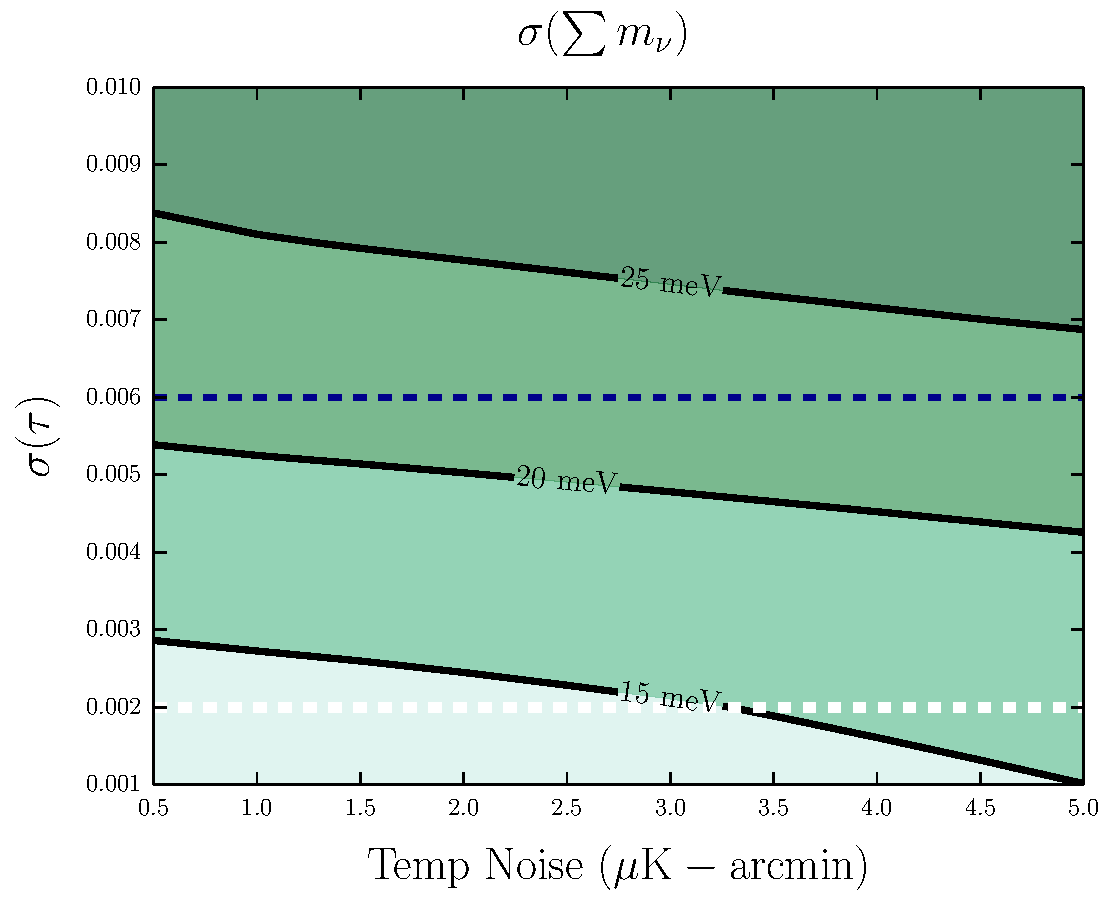
\includegraphics[width=0.45\textwidth]{figs/Mnu_tauprior.pdf}
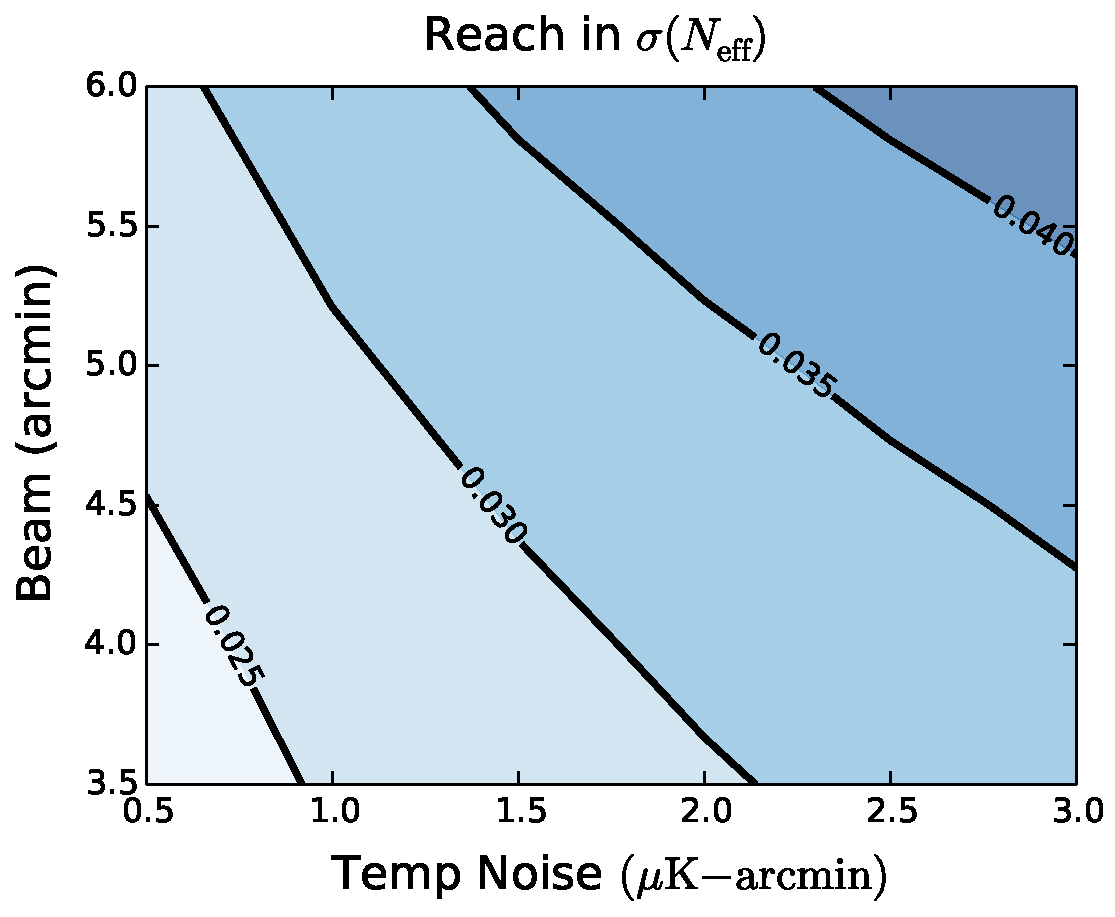
\includegraphics[width=0.45\textwidth]{figs/Neff_space.pdf}
\caption{ [Placeholders] {\it Left:} Neutrino mass constraints as a function of the prior on $\tau$.  {\it Right} $\Neff$ Forecasts as a function of resolution in arc-min and temperature noise in $\mu$K-arcmin assuming $f_{\rm sky} = 0.7$.}
\label{fig:Neff_future}
\end{center}
\end{figure}


